\documentclass[portrait,a0paper,fontscale=0.277]{baposter}

\usepackage{amsmath}
\usepackage{amssymb}
\usepackage{relsize}
\usepackage{graphicx}
\usepackage{enumitem}

%%%%%%%%%%%%%%%%%%%%%%%%%%%%%%%%%%%%%%%%%%%%%%%%%%%%%%%%%%%%%%%%%%%%%%%%%%%%%%%%
% save space in lists. Use this after the opening of the list
\newcommand{\compresslist}{%
\setlength{\itemsep}{0pt}%
\setlength{\parskip}{0pt}%
\setlength{\parsep}{0pt}%
}

% all the graphics are placed inside images folder
\graphicspath{{./images/}}

\begin{document}
\begin{poster}%
 % poster Options
 {
  % show grid to help with alignment
  grid=false,
  % column spacing
  colspacing=1em,
  % color style
  borderColor=cyan!30!white!90!black,
  headerColorOne=cyan!20!white!90!black,
  % format of textbox
  textborder=faded,
  % format of text header
  headerborder=open,
  headershape=roundedright,
  headershade=plain,
  background=none,
  bgColorOne=cyan!10!white,
  headerheight=0.12\textheight
 }
 % eye catcher
 % first logo
 {
\includegraphics[height=6em]{images/logo/kyutech}}
 % title
 {\bf\huge Quantitative Evaluation of Clothing Assistance using Whole-Body Robotic Simulator of the Elderly\vspace{1ex}}
 % authors
 {R.~P.~Joshi$^1$, T.~Shibata$^1$, K.~Ogata$^2$ and Y.~Matsumoto$^2$\vskip1ex
  {\small $^1$Kyushu Institute of Technology, Japan~|~$^2$National Institute of Advanced Industrial Science and Technology, Japan}}
 % second logo
 {
  
\includegraphics[height=3em]{images/logo/aist}
 }

 %%%%%%%%%%%%%%%%%%%%%%%%%%%%%%%%%%%%%%%%%%%%%%%%%%%%%%%%%%%%%%%%%%%%%%%%%%%%%%
 \headerbox{Background}{name=background,column=0,span=2,row=0}{
  \begin{minipage}{.4\linewidth}
   \begin{center}
    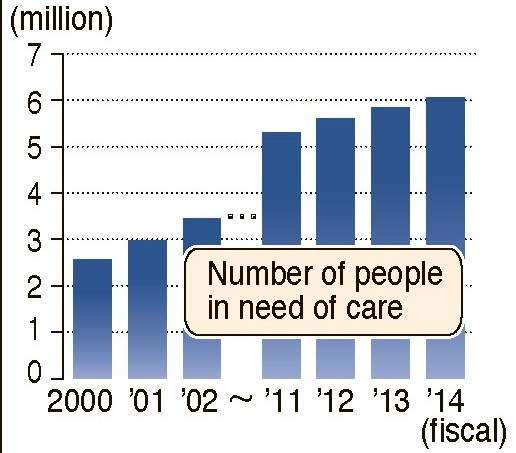
\includegraphics[width=.5\linewidth]{background/nursing_care}\\
    Demand of caregivers in Japan
   \end{center}
  \end{minipage}%
  \begin{minipage}{.58\linewidth}
   The robotic solutions to clothing assistance can significantly improve ADL for the elderly and disabled, because-
   \begin{itemize}\compresslist
    \item Most of the developed countries, including Japan, are aging rapidly.
    \item Use of caregiver is predominant in dressing ADL.
    \item Japan is facing a severe shortage of caregivers.
   \end{itemize}
  \end{minipage}
 }

 %%%%%%%%%%%%%%%%%%%%%%%%%%%%%%%%%%%%%%%%%%%%%%%%%%%%%%%%%%%%%%%%%%%%%%%%%%%%%%
 \headerbox{Introduction}{name=introduction,column=2,row=0}{
  \begin{itemize}[leftmargin=*]\compresslist
   \item We have developed a clothing assistance robot using dual arms.
   \item We could not systematically evaluate its performance because human arms are occluded.
   \item We propose to use another robot, Whole-Body Robotic Simulator of the Elderly.
  \end{itemize}
  \vskip2ex
 }

 %%%%%%%%%%%%%%%%%%%%%%%%%%%%%%%%%%%%%%%%%%%%%%%%%%%%%%%%%%%%%%%%%%%%%%%%%%%%%%
 \headerbox{Robotic Simulator for Elderly}{name=simulator,column=0,span=2,below=background}{
  \begin{minipage}{.55\linewidth}
   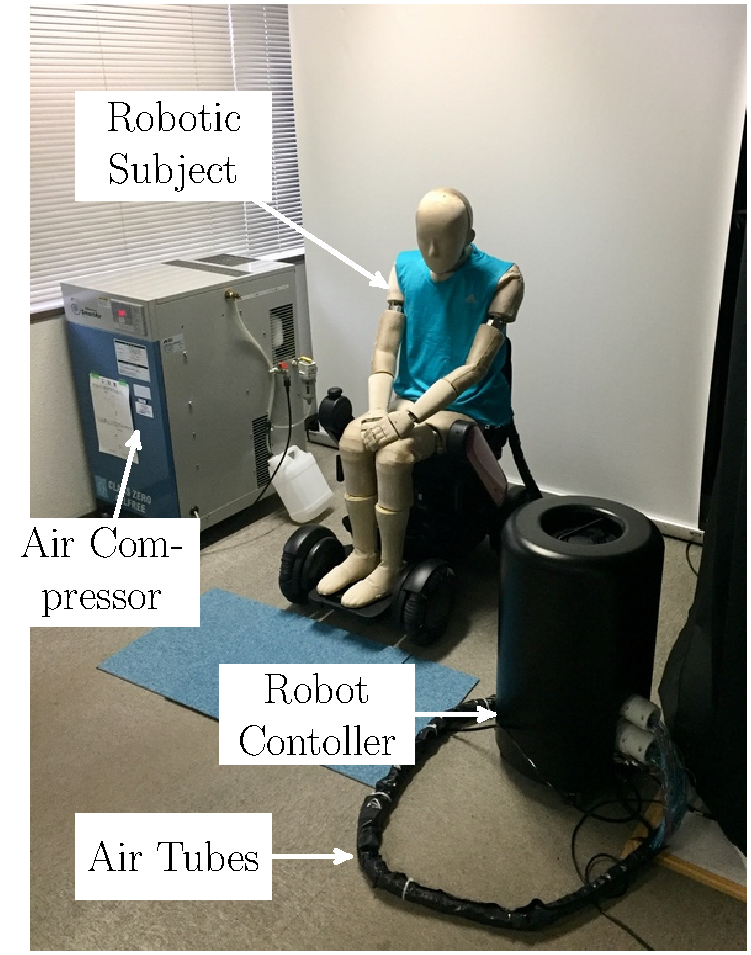
\includegraphics[width=.48\linewidth]{robotic_subject_setup/figure}
   \hskip4ex
   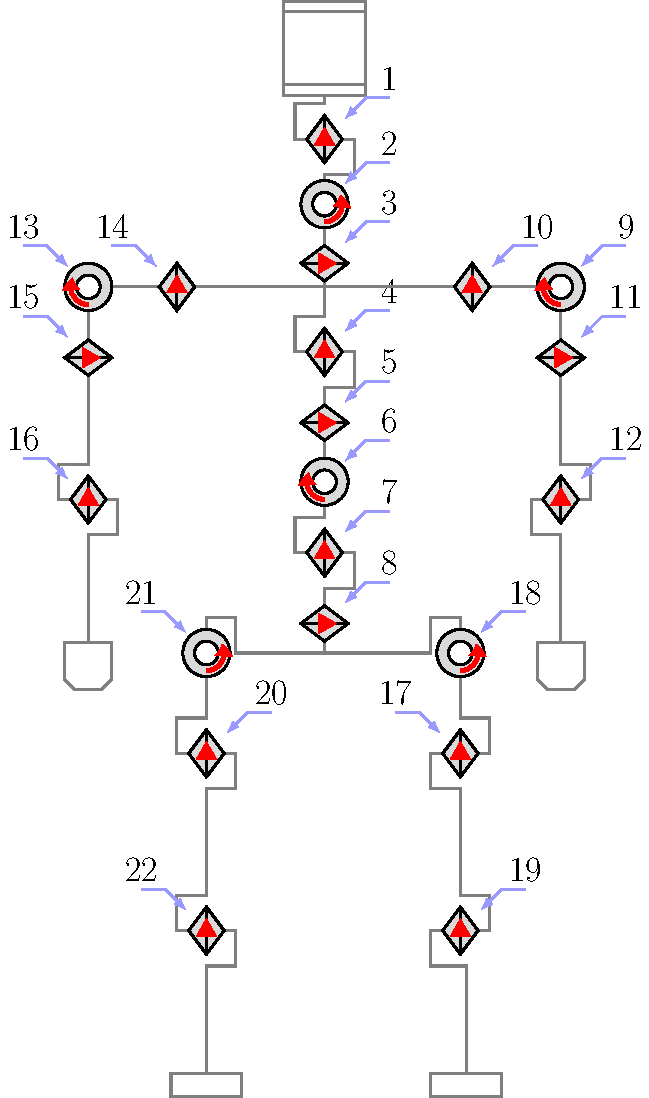
\includegraphics[width=.35\linewidth]{robotic_subject_model/figure}
  \end{minipage}%
  \begin{minipage}{.45\linewidth}
   \begin{itemize}\compresslist
    \item It can mimic the posture and movement of the elderly person during the dressing task.
    \item It is covered with a skin-like soft material.
    \item It has 28 passive and 22 active joints that are position controlled.
    \item Each active joint is pneumatically controlled. The air pressure is about 8 atm.
   \end{itemize}
  \end{minipage}
 }

 %%%%%%%%%%%%%%%%%%%%%%%%%%%%%%%%%%%%%%%%%%%%%%%%%%%%%%%%%%%%%%%%%%%%%%%%%%%%%%
 \headerbox{Experimental Setup}{name=setup,column=2,below=background}{
  \begin{center}
   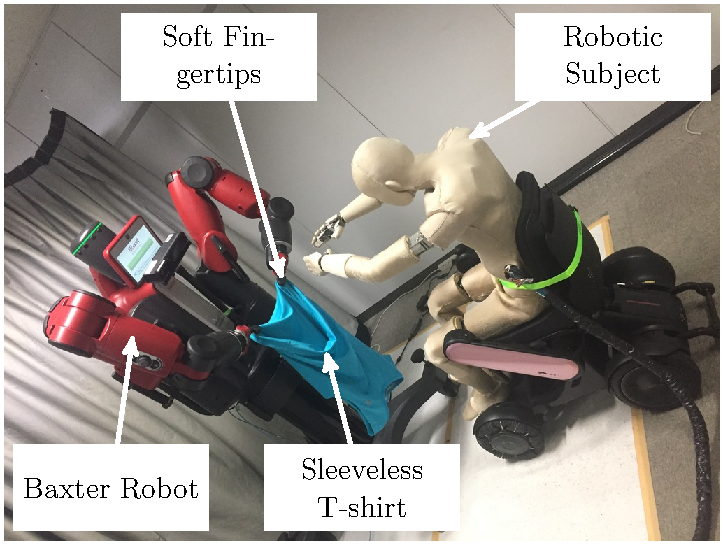
\includegraphics[width=.95\linewidth]{setup/figure}
  \end{center}
  \vskip1ex
 }

 %%%%%%%%%%%%%%%%%%%%%%%%%%%%%%%%%%%%%%%%%%%%%%%%%%%%%%%%%%%%%%%%%%%%%%%%%%%%%%
 \headerbox{DMP}{name=dmp,column=0,below=simulator}{
  It is used to learn the robot trajectory from demonstration.
  The policy is represented by a non-linear dynamical system as-
  \vskip-5mm
  \begin{equation*}
   \tau \dot{v} = K (x_g - x) -D v - K (x_g - x_0) s + K f(s).
  \end{equation*}
  $f(s) = \frac{\Sigma_{i} w_i \psi_i(s)}{\Sigma_{i} \psi_i(s)} s$ and $\psi_i$ is a Gaussian basis function.

  \vskip1ex
  We redefine $f(s)$ so that it allows to modify the start and goal state, i.e., $x_0$ and $x_g$ respectively.
  \vskip-5mm
  \begin{equation*}
   f_{target}(s) = \frac{D v + \tau \dot{v}}{K} - (x_g - x) +  (x_g - x_0) s
  \end{equation*}
 }

 %%%%%%%%%%%%%%%%%%%%%%%%%%%%%%%%%%%%%%%%%%%%%%%%%%%%%%%%%%%%%%%%%%%%%%%%%%%%%%
 \headerbox{Method}{name=method,column=1,span=2,below=simulator}{
  \begin{minipage}{.45\linewidth}
   Our method contains three stages-
   \begin{enumerate}[leftmargin=4ex]\compresslist
    \item Demonstration
    \item Training
    \item Testing
   \end{enumerate}
  \end{minipage}

  \vskip-18mm
  \hfill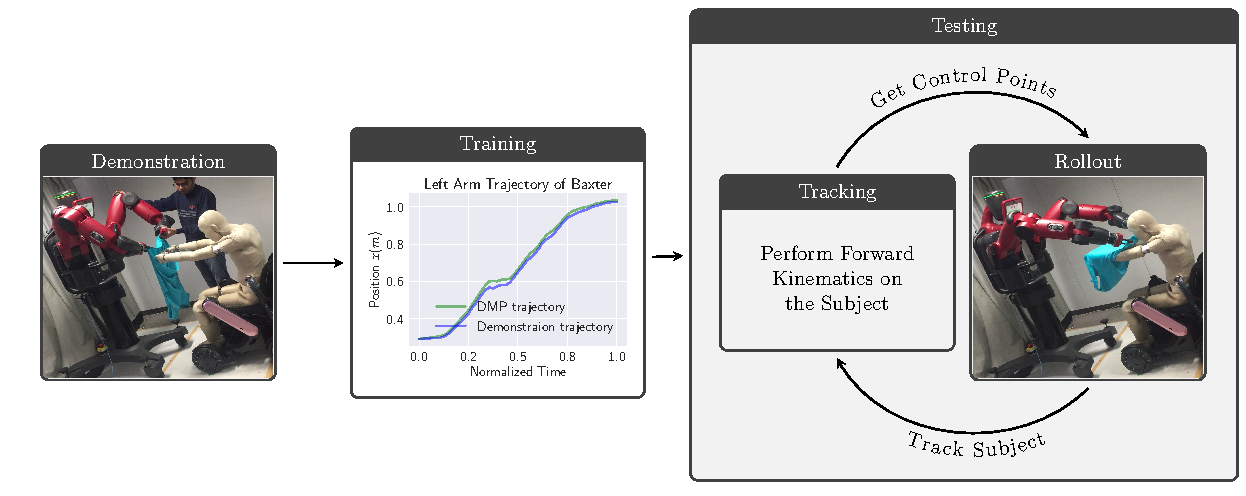
\includegraphics[clip, trim=6mm 2mm 1mm 1mm, width=.8\linewidth]{method/figure}

  \vskip-2mm
  The start and goal (control) points of DMP are the\\
  fingertips and elbows of the robotic subject, respectively.
 }

 %%%%%%%%%%%%%%%%%%%%%%%%%%%%%%%%%%%%%%%%%%%%%%%%%%%%%%%%%%%%%%%%%%%%%%%%%%%%%%
 \headerbox{Results}{name=results,column=0,span=3,below=dmp}{
  We empirically defined two types of arm movements of the robotic subject.
  These movements belong to day-to-day arm stretching movements.

  \vskip2ex
  \begin{minipage}[t]{.48\linewidth}
   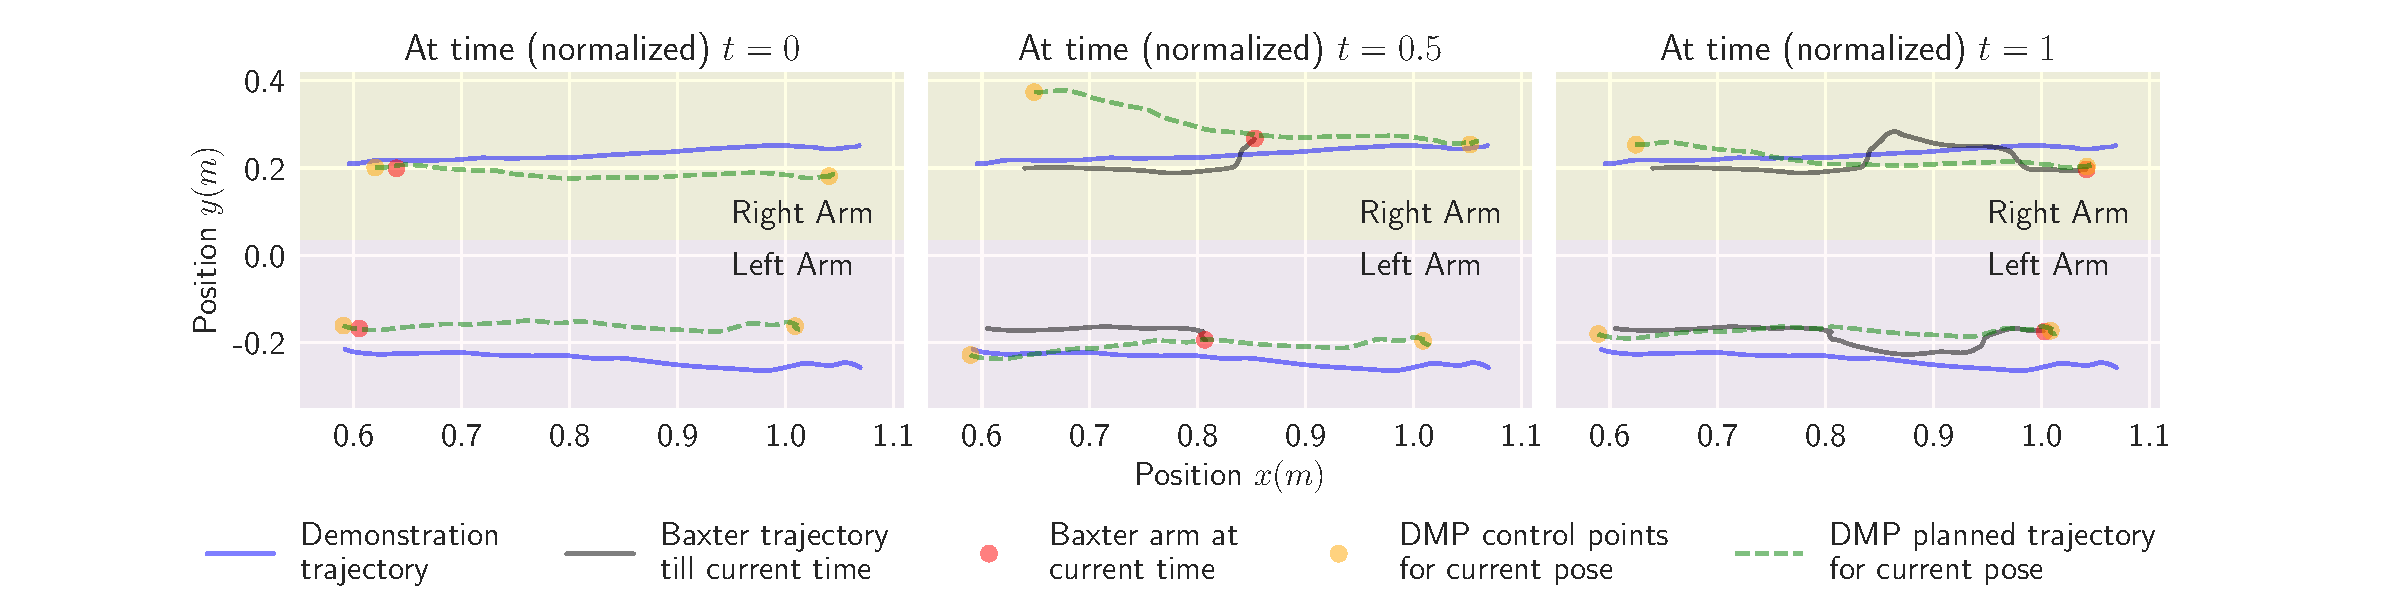
\includegraphics[trim={32mm 3mm 39mm 5mm}, clip, width=\linewidth]{robot_and_dmp_trajectories/dmp}
  \end{minipage}
  \hskip4ex
  \begin{minipage}[t]{.48\linewidth}
   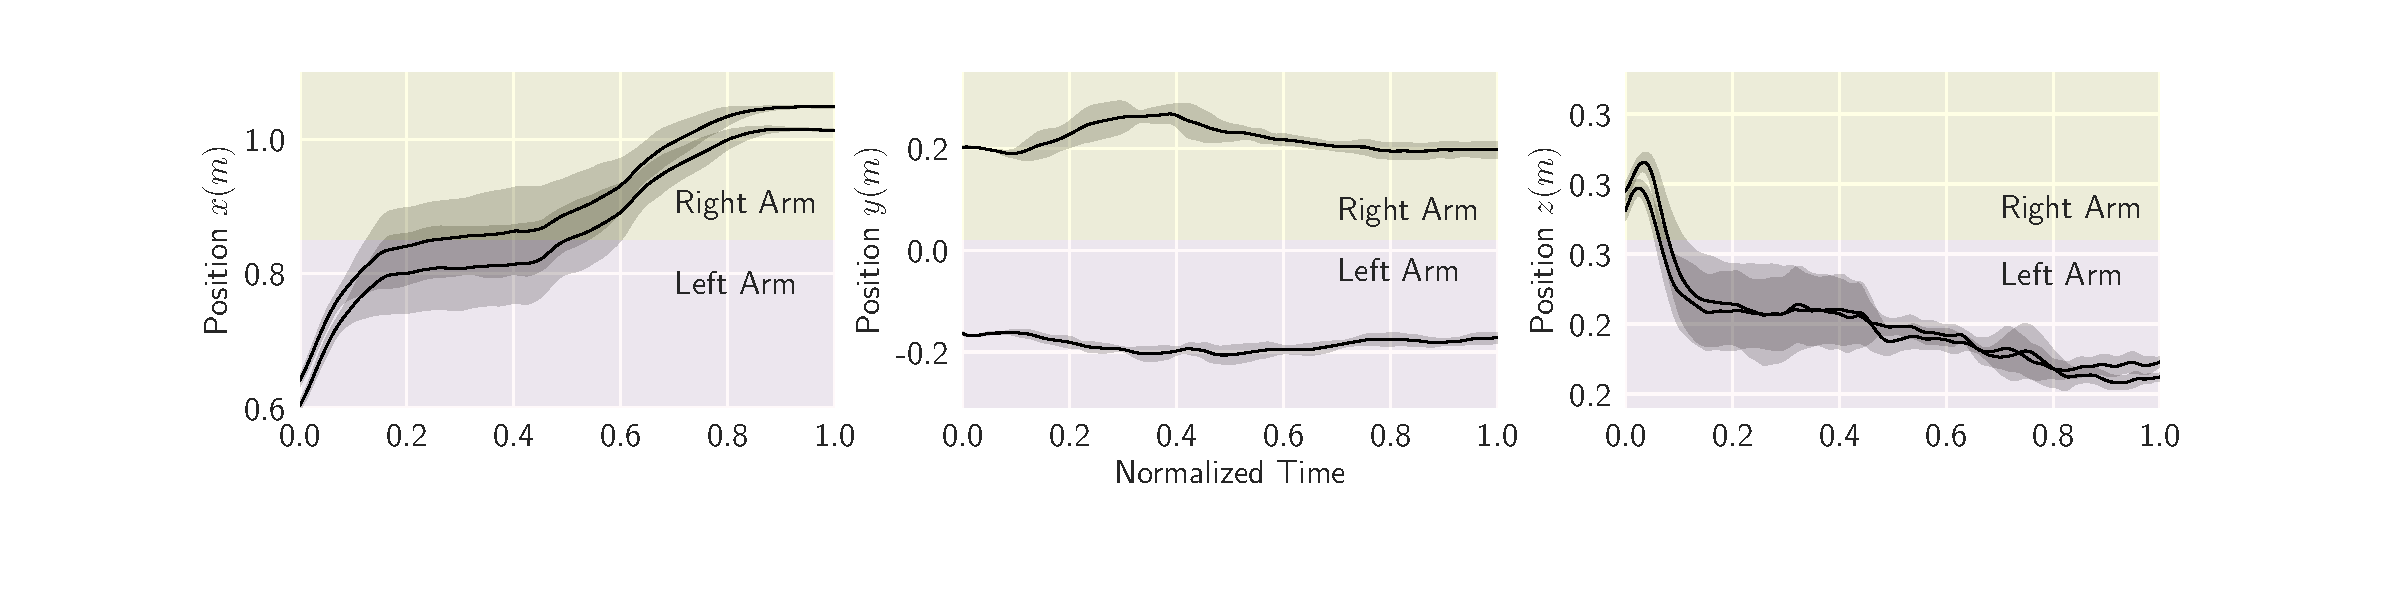
\includegraphics[trim={34mm 3mm 37mm 11mm}, clip, width=\linewidth]{robot_and_dmp_trajectories/baxter}
  \end{minipage}

  \hfill

  \begin{minipage}[t]{.48\linewidth}
   \begin{itemize}\compresslist
    \item The Baxter robot is commanded at each timestamp while setting the control points on the fly.
    \item At $t = 0.5$, both the arms of the Baxter robot are adopting the change and moving away from each other.
   \end{itemize}
  \end{minipage}
  \hskip4ex
  \begin{minipage}[t]{.48\linewidth}
   \begin{itemize}\compresslist
    \item We ran the arm dressing task ten times and visualized the robot trajectory.
    \item The y and z-axis of Baxter confirm that the arms of the robotic subject are not in symmetry.
   \end{itemize}
  \end{minipage}
 }

 %%%%%%%%%%%%%%%%%%%%%%%%%%%%%%%%%%%%%%%%%%%%%%%%%%%%%%%%%%%%%%%%%%%%%%%%%%%%%%
 \headerbox{Conclusion}{name=conclusion,column=0,below=results}{
  \begin{itemize}[leftmargin=*]\compresslist
   \item Systematic evaluation is necessary to make such devices accessible in the elderly care facilities.
   \item We have shown the plausibility of our approach by performing the dressing task on defined arm movements.
  \end{itemize}
 }

 %%%%%%%%%%%%%%%%%%%%%%%%%%%%%%%%%%%%%%%%%%%%%%%%%%%%%%%%%%%%%%%%%%%%%%%%%%%%%%
 \headerbox{Future Work}{name=futurework,column=1,below=results}{
  \begin{itemize}[leftmargin=*]\compresslist
   \item Incorporating 3-dimensional arm movements, head, and torso movements.
   \item Perform complete dressing, i.e., right from fingertip through the head till waist.
   \item Experimentation with the elderly and understand their psychological behavior too.
  \end{itemize}
 }

 %%%%%%%%%%%%%%%%%%%%%%%%%%%%%%%%%%%%%%%%%%%%%%%%%%%%%%%%%%%%%%%%%%%%%%%%%%%%%%
 \headerbox{References}{name=references,column=2,below=results}{
  \smaller
  \bibliographystyle{ieee}
  \renewcommand{\section}[2]{}
  \begin{thebibliography}{1}\itemsep=0em
   \setlength{\baselineskip}{0.4em}
   \bibitem{matsumoto2018evaluating}
   Y.~Matsumoto, K.~Ogata, I.~Kajitani, K.~Homma, and Y.~Wakita.
   \newblock {Evaluating Robotic Devices of Non-Wearable Transferring Aids Using Whole-Body Robotic Simulator of the Elderly}.
   \newblock In {\em IROS'18}.
   \bibitem{joshi2019framework}
   R.~P.~Joshi, N.~Koganti, and T.~Shibata.
   \newblock {A Framework for Robotic Clothing Assistance by Imitation Learning}.
   \newblock In {\em Advanced Robotics'19}.
  \end{thebibliography}
 }
\end{poster}
\end{document}
